\chapter{Loewner Evolutions of Anisotropic Systems}
\label{ch6-asle}

In this work we take the effort to relate the Stochastic Loewner Evolution with
strongly anisotropic systems. Because such systems are not conformally
invariant, the driving process of these models must not be a simple Brownian
motion.

\section{Lévy Flights and Schramm-Loewner Evolutions}

One possible source of anisotropy in the context of SLE is the presence of
anomalous diffusion in the driving process. A stochastic process $X_t$ is
said to display anomalous diffusion if the mean squared displacement
behaves asymptotically as
\begin{equation}
    \left\langle X_t^2 \right\rangle \sim bt^\alpha
\end{equation}
with $\alpha\neq 1$. Processes that have $\alpha < 1$ are called subdiffusive
models and those with $\alpha > 1$ are called superdiffusive.

There are several models that present anomalous diffusion. Rushkin et Al [..]
proposed using L\'evy-flights as a driving process. L\'evy-flights are defined as
processes that have jump size distributed as a power law, that is
\begin{equation}
    P(X_{t+dt} - X_t \in [x, x+dx]) \propto \frac{1}{|x|^{1+\mu}}dxdt
\end{equation}
They've shown that Loewner Evolutions drive by such processes behave


\section{Generating Large Percolation Traces}
\label{sec:hulls}

Simulating the percolation process and extracting the percolating cluster
perimeter is very straightforward and a number of good algorithms are
available. However, because of the spotty behavior of the zipper algorithm
(see Fig.~\ref{fig:euzip}) in the high $\kappa$ ($>4$) domain, we need very
large traces in order to obtain reliable results.

The usual algorithms are normally very memory hungry because you need to store
the state of all sites in the lattice. Since we are only interested in
obtaining the perimeter of the percolating cluster, which consists of only a
small portion of the lattice, one might imagine if there's a more efficient way
of simulating these curves. Luckily there is, thanks to the locality property
of the percolation model. The method is called the \textit{percolation
exploration process}.

The exploration process is easier to define in the triangular lattice, because
at any given time the walker is always facing a single site, unlike the square
lattice, in which it faces two sites at once, complicating things a little (it
doesn't make it impossible, though). In the exploration process, a walker is
put in an initial position at the bottom of the lattice. The walker observes
the state of the site right in front of him. If it is unoccupied, the walker
turns clockwise, otherwise it turns clockwise. Then the walker takes a step in
the direction it is facing. The algorithm guarantees that the curve will not
self-intersect and will not get trapped.

Because we restrict ourselves to chordal SLE, the walker can never leave the
upper-half plane. To assure this, we impose closed boundary conditions in which
the left side of the bottom row of the lattice is always unoccupied and the
right side is always occupied. This way the trace will always turn away from
the real line.

It's pretty clear the advantage of this method, you only need to store the
information about the sites directly adjacent to the perimeter, which can be
cached in your container of preference, like a hash table (also known as maps
or dictionaries). This allow us to simulate traces with up to million points.
In fact we could easily go above that, the limiting factor being the time the
zipper algorithm takes to compute the driving function.

\begin{figure}
\begin{center}
    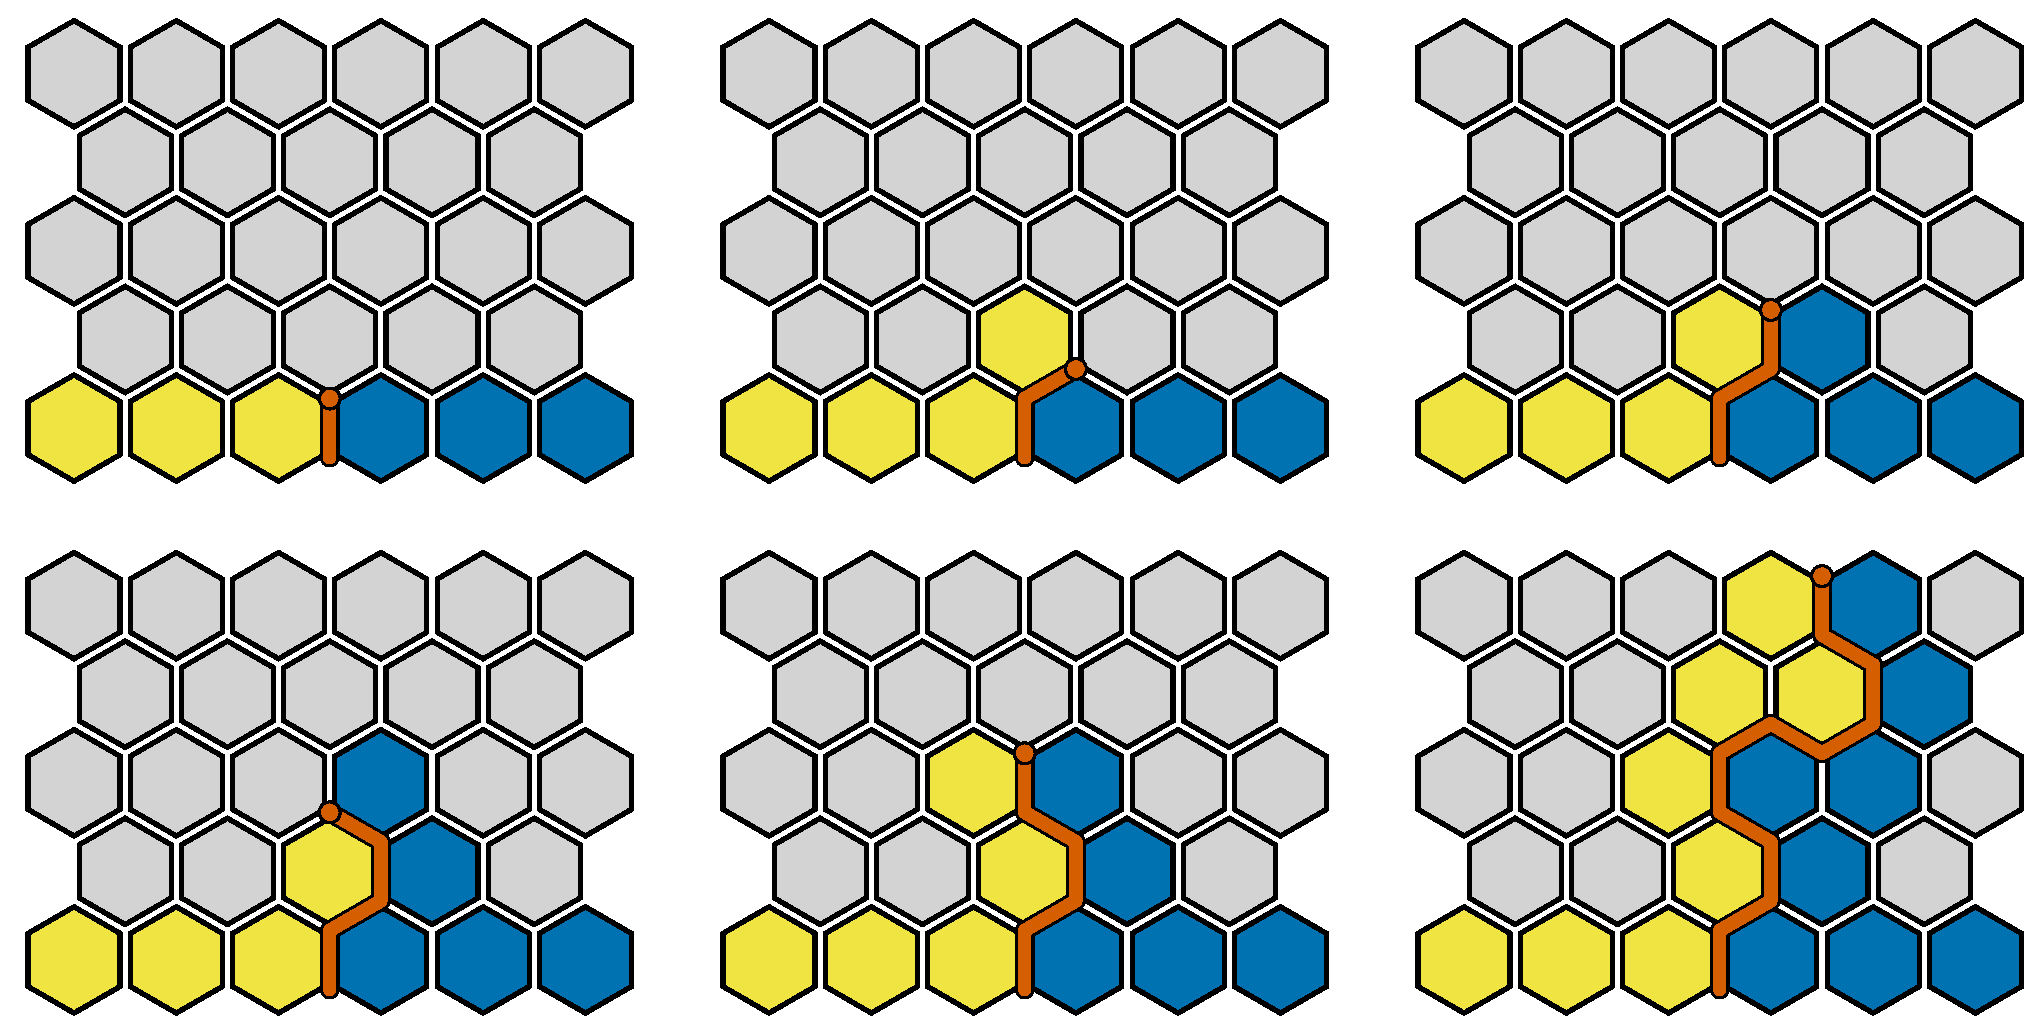
\includegraphics[scale=0.45]{chapters/ch6-asle/figs/explore}
\end{center}
\caption{The first few steps of a percolation exploration process with closed
    boundary conditions in a triangular lattice, which means the left side of
    the bottom row is always unoccupied (yellow) and the right side is always
    occupied (blue). At each step, the walker checks the status of the site
    right in front of it. If it is yellow, the walker turns clockwise and takes
    a step. If it is blue it turns counter-clockwise before taking a step. This
    method is superior because you only need to store the information about the
    sites adjacent to the curve, saving RAM and allowing for simulations of
    very large traces.}
\label{fig:explore}
\end{figure}


\section{Detrended Fluctuation Analysis}
\label{sec:dfa}

We want to test whether or not the driving functions present long range
correlations. Other works have shown that some form of anisotropy can be
observed in SLE traces driven by L\'evy Flights. We have good reasons to
believe this is not the case for multi-layered and directed percolation,
because L'evy flights do not show subdiffusion and they generate discontinuous
traces.

In order to close the issue we perform one last test: check for the presence of
long range correlations. To do that we employ a method called Detrended
Fluctuation Analysis (DFA for short), which is an adaptation of an older
algorithm called simply Fluctuation Analysis. It is specially designed for the
analysis of non stationary series.%~\cite{Peng1994,Hardstone2012}.

Given a time series of $N$ data points $\{x_i\}$, we first generate a random walk
out of it by making the cumulative profile of the series
\begin{equation}
    X_i = \sum_{i=1}^{N} \left({x_i - \left\langle x \right\rangle}\right).
\end{equation}
The accumulated series is then divided in $m$ non overlapping partitions, each with
$s = N/m$ elements. In case $N$ is not divisible by $m$ we can still make use
of the last elements of the series by taking $s=\left\lfloor N/m\right\rfloor$
and reflecting it in the end the following way
\begin{equation}
    X\rightarrow\left\{X_1, \ldots, X_{ms},
                       X_{N}, X_{N - 1}, \ldots,
                       X_{N - ms}\right\}.
\end{equation}
In this case we actually changed the series size to $N\rightarrow2ms$ and the
number of intervals to $m\rightarrow2m$, so this should be taken in account in
later equations. This step is optional, but useful in order to use all the
information embedded in the time series.

We then determined the trend of each partition by fitting them separately using
a polynomial of degree $v$. Usually a first or second degree polynomial is
chosen. The series is detrended by taking the difference of the signal value and
the trend 
\begin{equation}
    Y_i = \sum_{i=1}^{N} X_i - f_v(i),
\end{equation}
where $f_v(i)$ is the value of the trend in the point $i$. We define the fluctuation
function as the standard deviation of the detrended signal, which is a function
of the number of points $s$ in each partition of the time series
\begin{equation}
    F(s) = \sqrt{\frac{1}{N}\sum_{i=1}^{N}Y_i}.
\end{equation}

A plot of $F(s)$ vs. $s$ in a log-log scale should show a straight line
for well a behaved series. %(see Fig.~\ref{fig:dfa}).
The Hurst exponent of the series can be determined by fitting the fluctuation
function with a power law
\begin{equation}
    F(s)\sim s^h.
\end{equation}

\begin{figure}[t]
    \begin{center}
        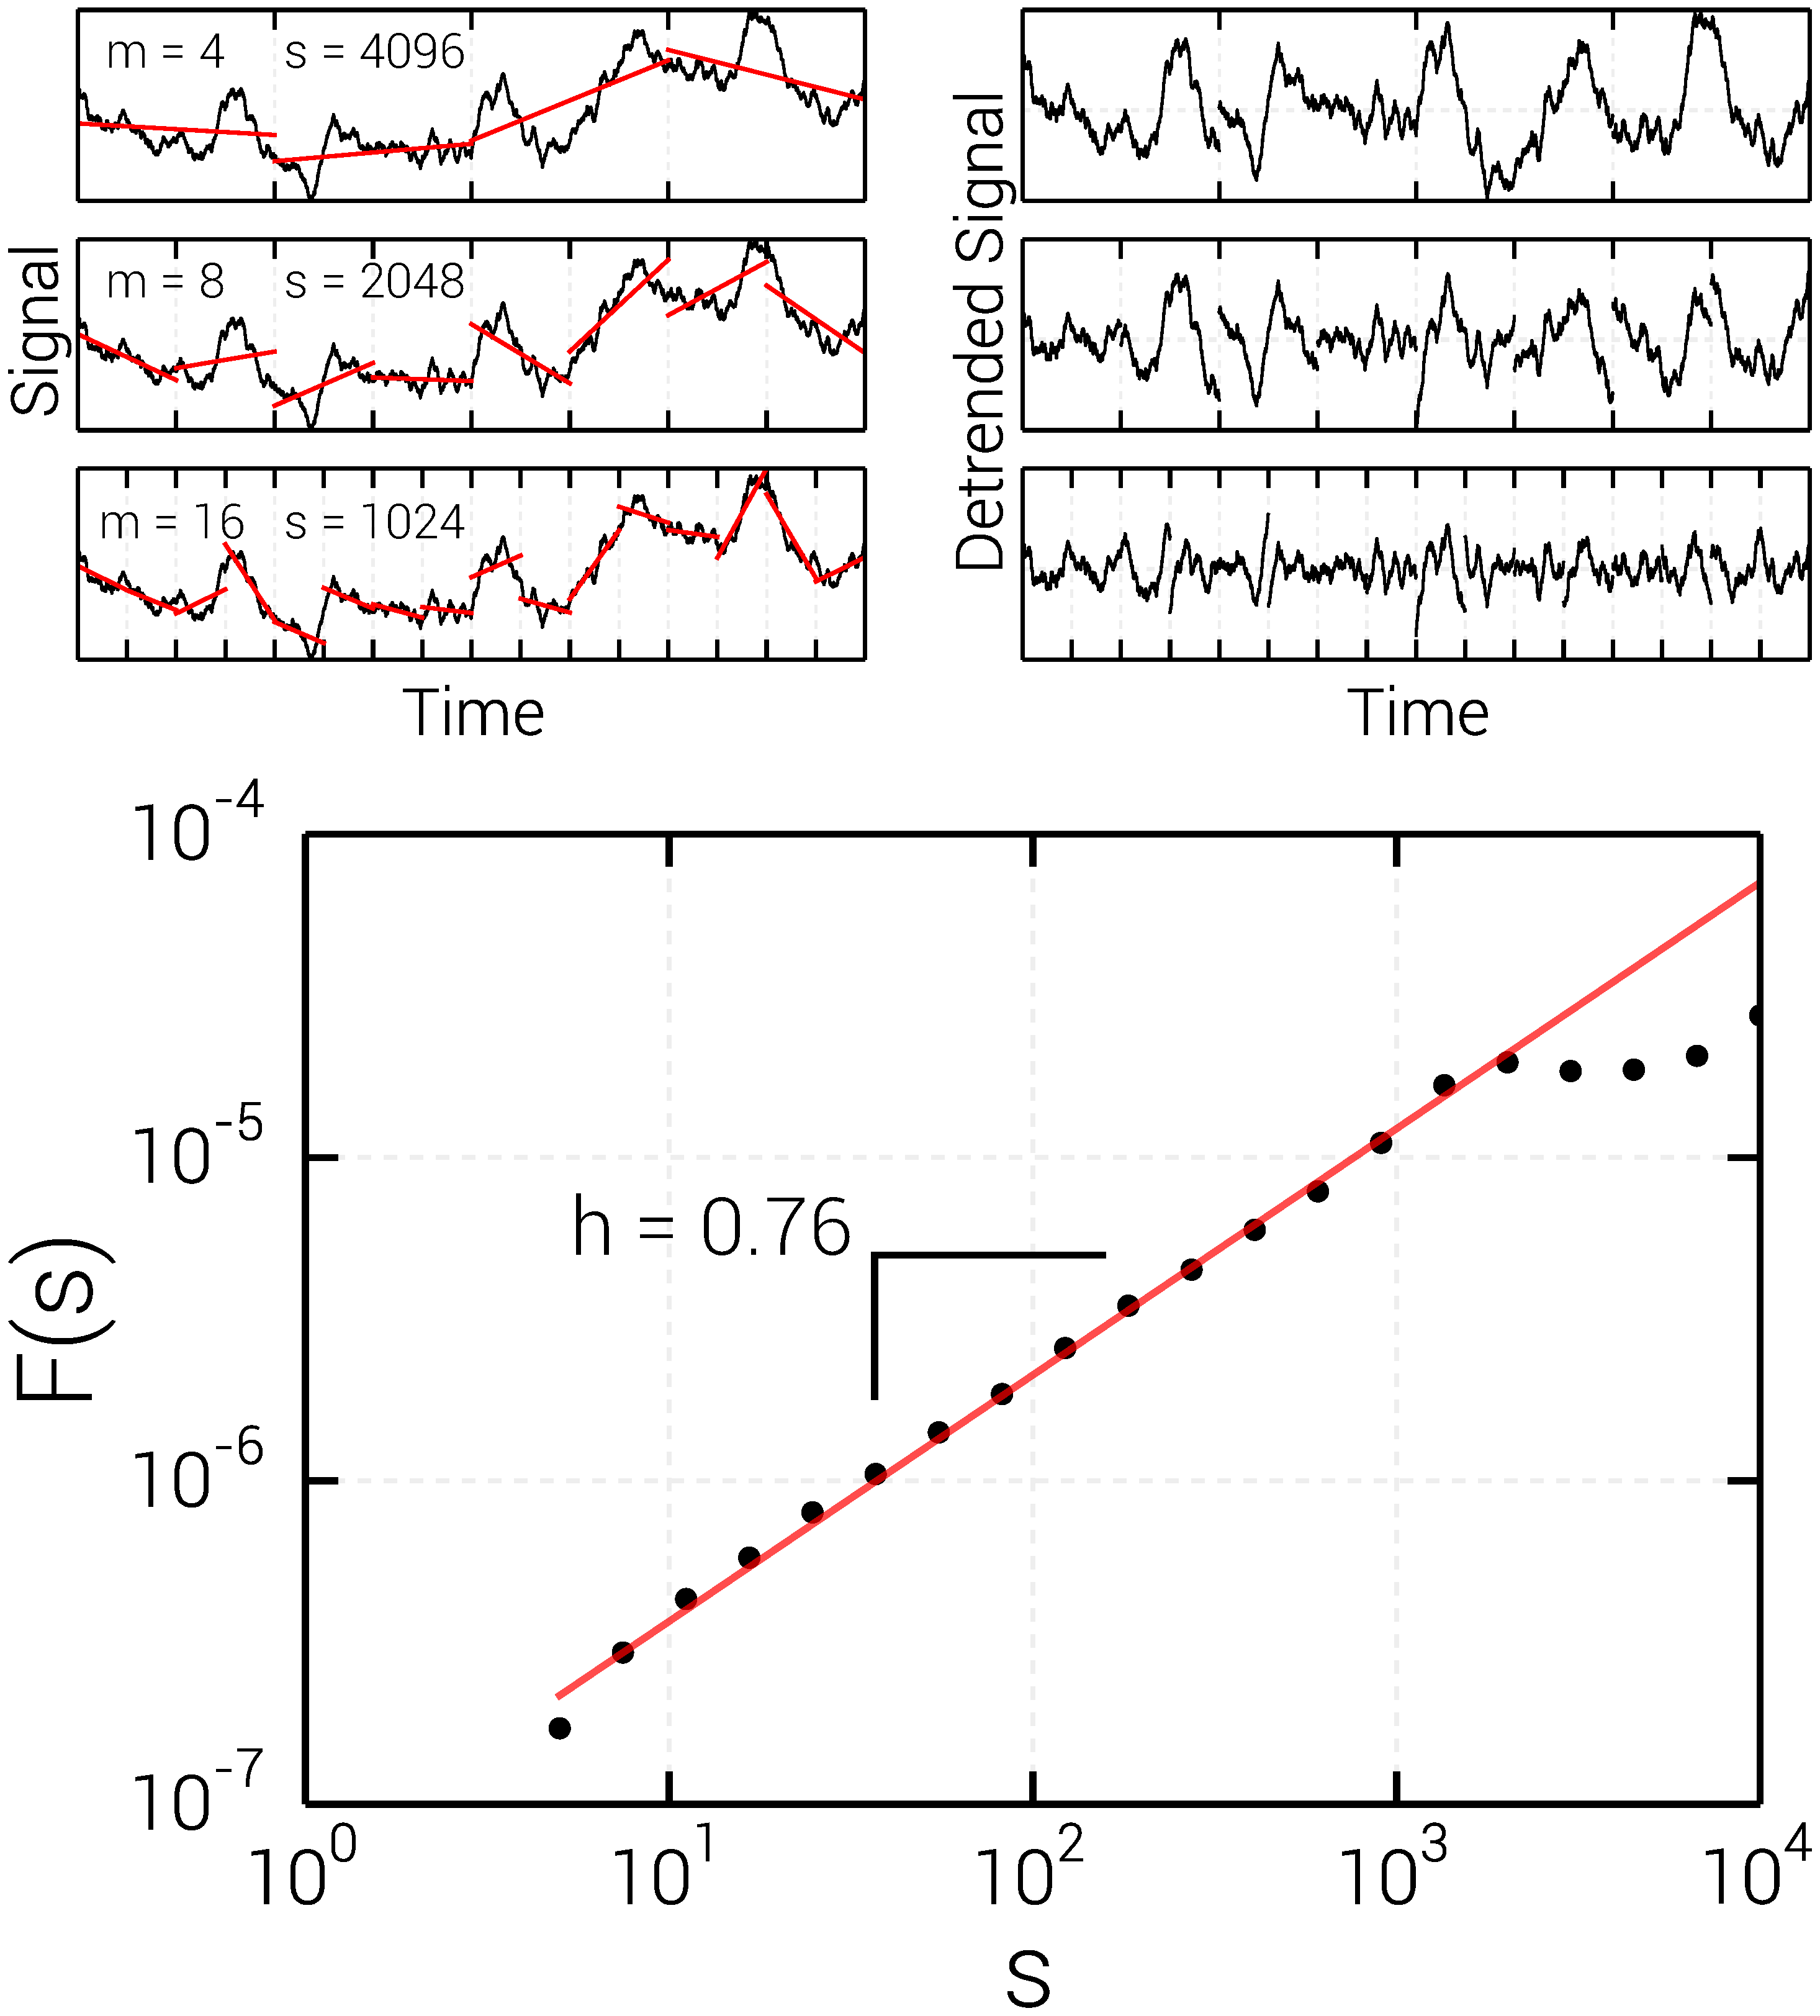
\includegraphics[scale=0.25]{chapters/ch6-asle/figs/dfa}
    \end{center}
    \caption{The Detrended Fluctuation Analysis (DFA) of a time series of
        $N=16,384$ data points. First we divided the series in $m$ partitions with
        $s$ points each (top-left), then fitted each separately with a first order
        polynomial $f_1(i)$ (red lines), obtaining the detrended series by subtracting
        the signal by the trend (top-right).  The fluctuation function (the standard
        deviation of the detrended signal) is computed for various values of $s$
        (bottom).  The Hurst exponent is then determined by fitting the fluctuation
        function with a power law $F(s)\sim s^h$.}
\label{fig:dfa}
\end{figure}

\begin{figure}
\begin{center}
    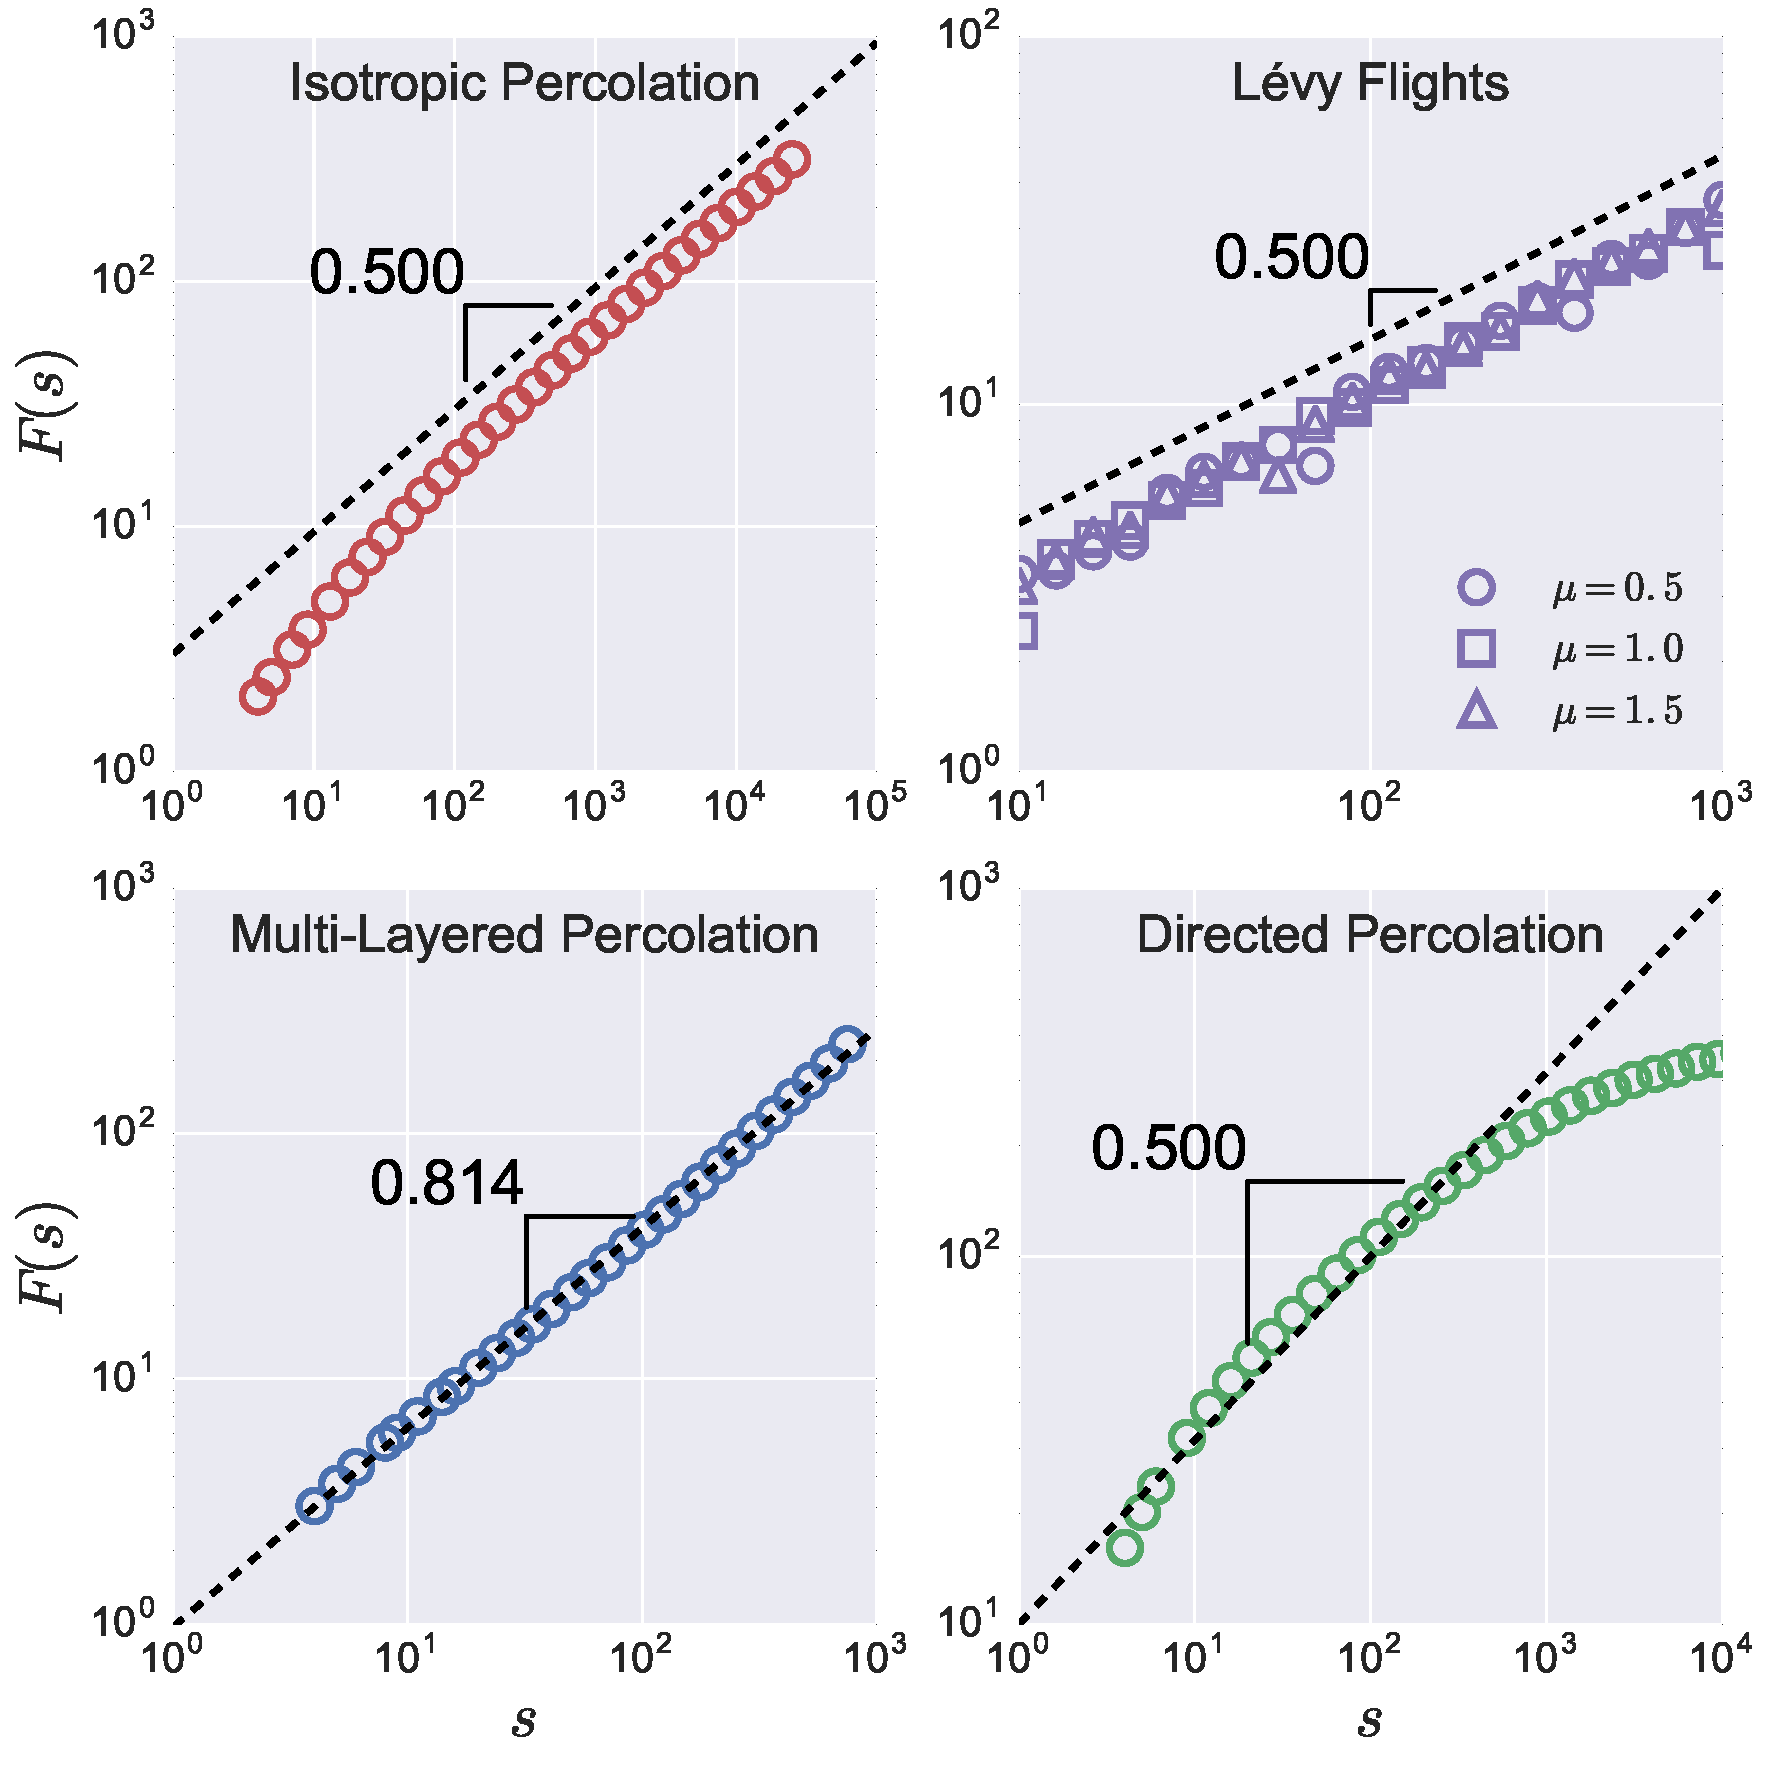
\includegraphics[scale=0.45]{chapters/ch6-asle/figs/dfaresults}
\end{center}
\caption{Results of detrended fluctuation analysis (DFA) of the driving
    functions of percolation models. As expected, the driving function of the
    isotropic percolation (top left) is a Brownian motion, therefore have
    $H=0.5$. For comparison the DFA of L\'evy flights with several $\alpha$ is
    shown (top right). Despite displaying anomalous diffusion, it still have
    $H=0.5$. Multi-layered percolation however shows a very distinct exponent
    $H=0.814$, which is consistent with the diffusion exponent shown inf
    Figure~[???]. The fluctuation function of directed percolation does not
    have a power-law behavior, which indicates that the series is.}
\label{fig:dfaresults}
\end{figure}



\section{Generating Fractional Browninan Motions}
\label{sec:fbm}

We want to generate fractional Brownian motions $B_t$ such that
\begin{equation}
    \label{eq:fbm}
    \left\langle B_t^2 \right\rangle = bt^{2H}.
\end{equation}
There are several methods to generate this process numerically, but not all of
them give you ample control over the prefactor $b$, although most are very
accurate in $H$. A method that adequately fulfills this criterion is the
Davies-Harte algorithm. It can be used to generate any stationary Gaussian
process for which the autocovariance sequence is known. In the case of
the fractional Brownian motion, it takes the form
\begin{equation}
    c_i = \frac{b}{2} \left(
            \left|i+1\right|^{2H} +
            \left|i-1\right|^{2H} -
            2\left|i\right|^{2H}
          \right)
\end{equation}

To obtain a series of length $N$ we generate the following sequence of $2N$
points
\begin{equation}
    s_i=\left\{c_{0},c_{1},\ldots,c_{N},c_{N-1},\ldots,c_{1}\right\}
\end{equation}
and compute its discrete Fourier transform, that is
\begin{equation}
    g_{i}=\sum_{j}s_{j}e^{-i\pi kj/N}.
\end{equation}
This operation can be done in $O(N\log N)$ operations using a fast Fourier
transform. The $g_i$ are real valued, but a necessary condition for the
Davies-Harte algorithm to work is that they also be nonnegative. It is
important to check for this condition even if just for debugging purposes,
as it catches a lot of small mistakes.

Let $W_{i\in[0,N]}$ be a sequence of $N+1$ random complex numbers where the
real and imaginary parts are independently distributed according to a normal
distribution with zero mean and unit variance. We then construct the series
\begin{equation}
    Y_{i\in[0,2N-1]}=\begin{cases}
        \sqrt{2Ng_{i}}\mbox{Re}\left\{ W_{i}\right\}  & \mbox{if } i=0,N\\
        \sqrt{Ng_{i}}W_{i} & \mbox{if } i\in\left[1, N-1\right]\\
        \sqrt{Ng_{i}}W_{2N-i}^{*} & \mbox{if } i\in\left[N+1, 2N-1\right]
    \end{cases},
\end{equation}
where $W^{*}$ is the complex conjugate. The fractional Brownian motion $B_t$ is
obtained by computing the inverse Fourier transform of this series. Although
the obtained series have $2N$ points we discard the second half, as it is not
guaranteed to be well behaved. The $B_t$ are defined for $t\in{0,1,\ldots,N-1}$,
but the series can easily be rescaled for any timespan desirable by applying
the relation
\begin{equation}
    B_{t\in[0,t_{f}]}={\left(\frac{t_{f}}{N}\right)}^{H}B_{t\in[0,N]}.
\end{equation}

In Figure~\ref{fig:fbm}, we show some examples of fractional Brownian motion
generated using this algorithm. We also show that the mean squared displacement
behaves as described by Eq.~\ref{eq:fbm}.

\begin{figure}
\begin{center}
    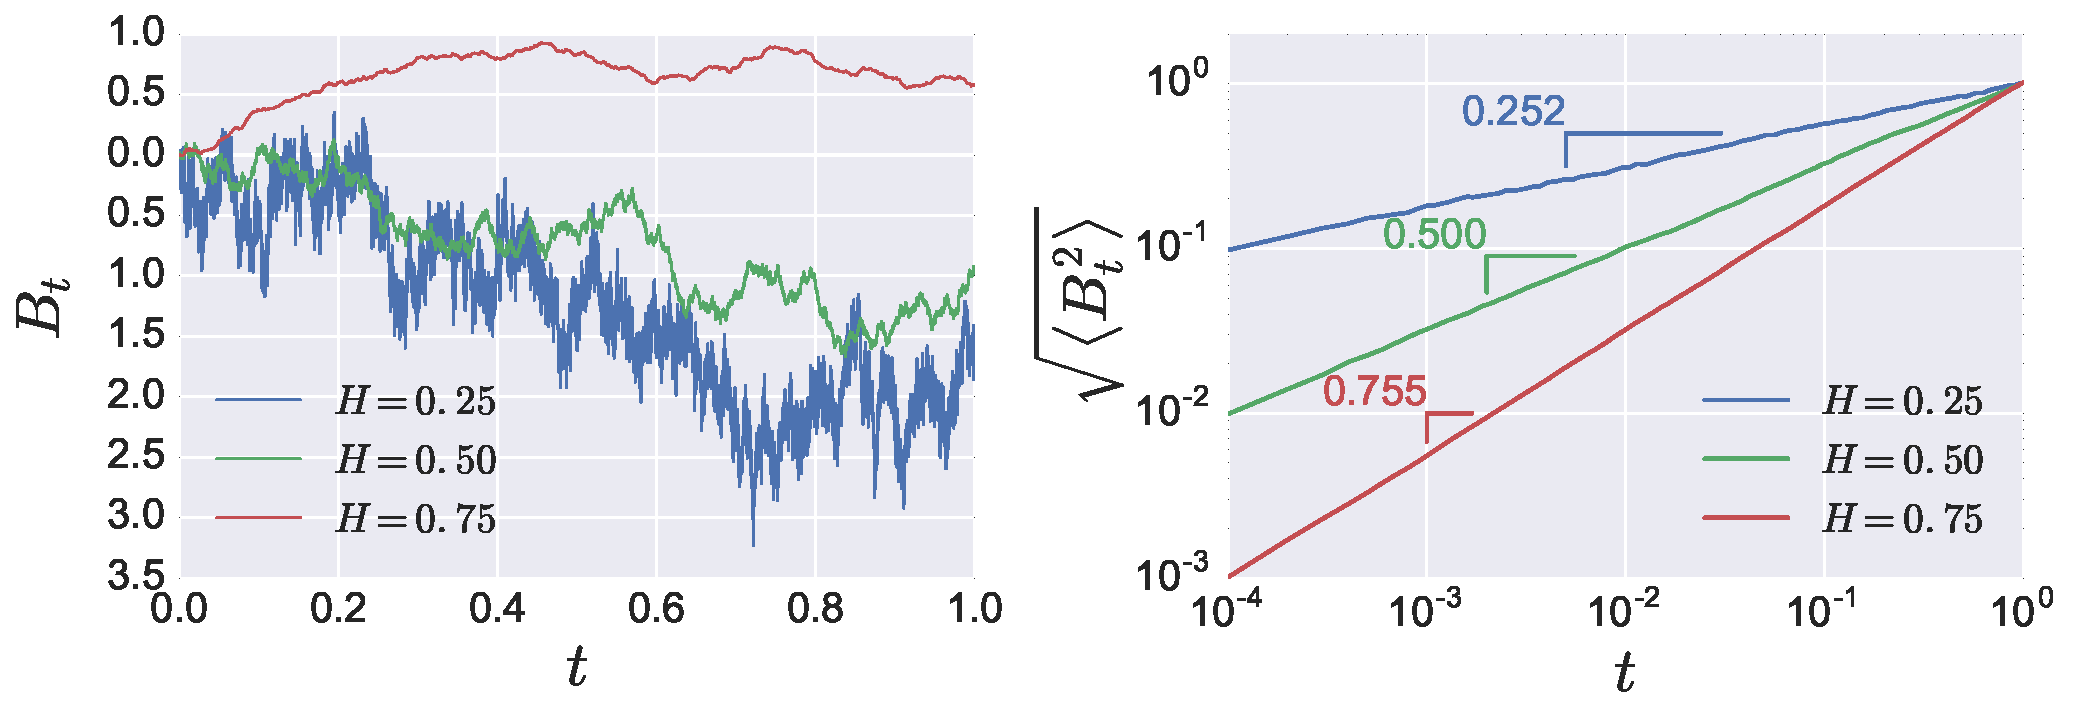
\includegraphics[scale=0.45]{chapters/ch6-asle/figs/fbm}
\end{center}
\caption{Example of three fractional Brownian motions generated using the
    Davies-Harte algorithm (left). They all have $b=1.0$ and different values
    of $H$. We also show the behavior of the mean square displacement of the
    scaling properties of the curves. We found that the mean square displacement
    scales as $\sqrt{\left\langle B_t^2\right\rangle}=\sqrt{b}t^H$ with
    parameters very similar to the input given.}
\label{fig:fbm}
\end{figure}


\section{Scaling Analysis}
\label{sec:scaling}

\begin{figure}
\begin{center}
    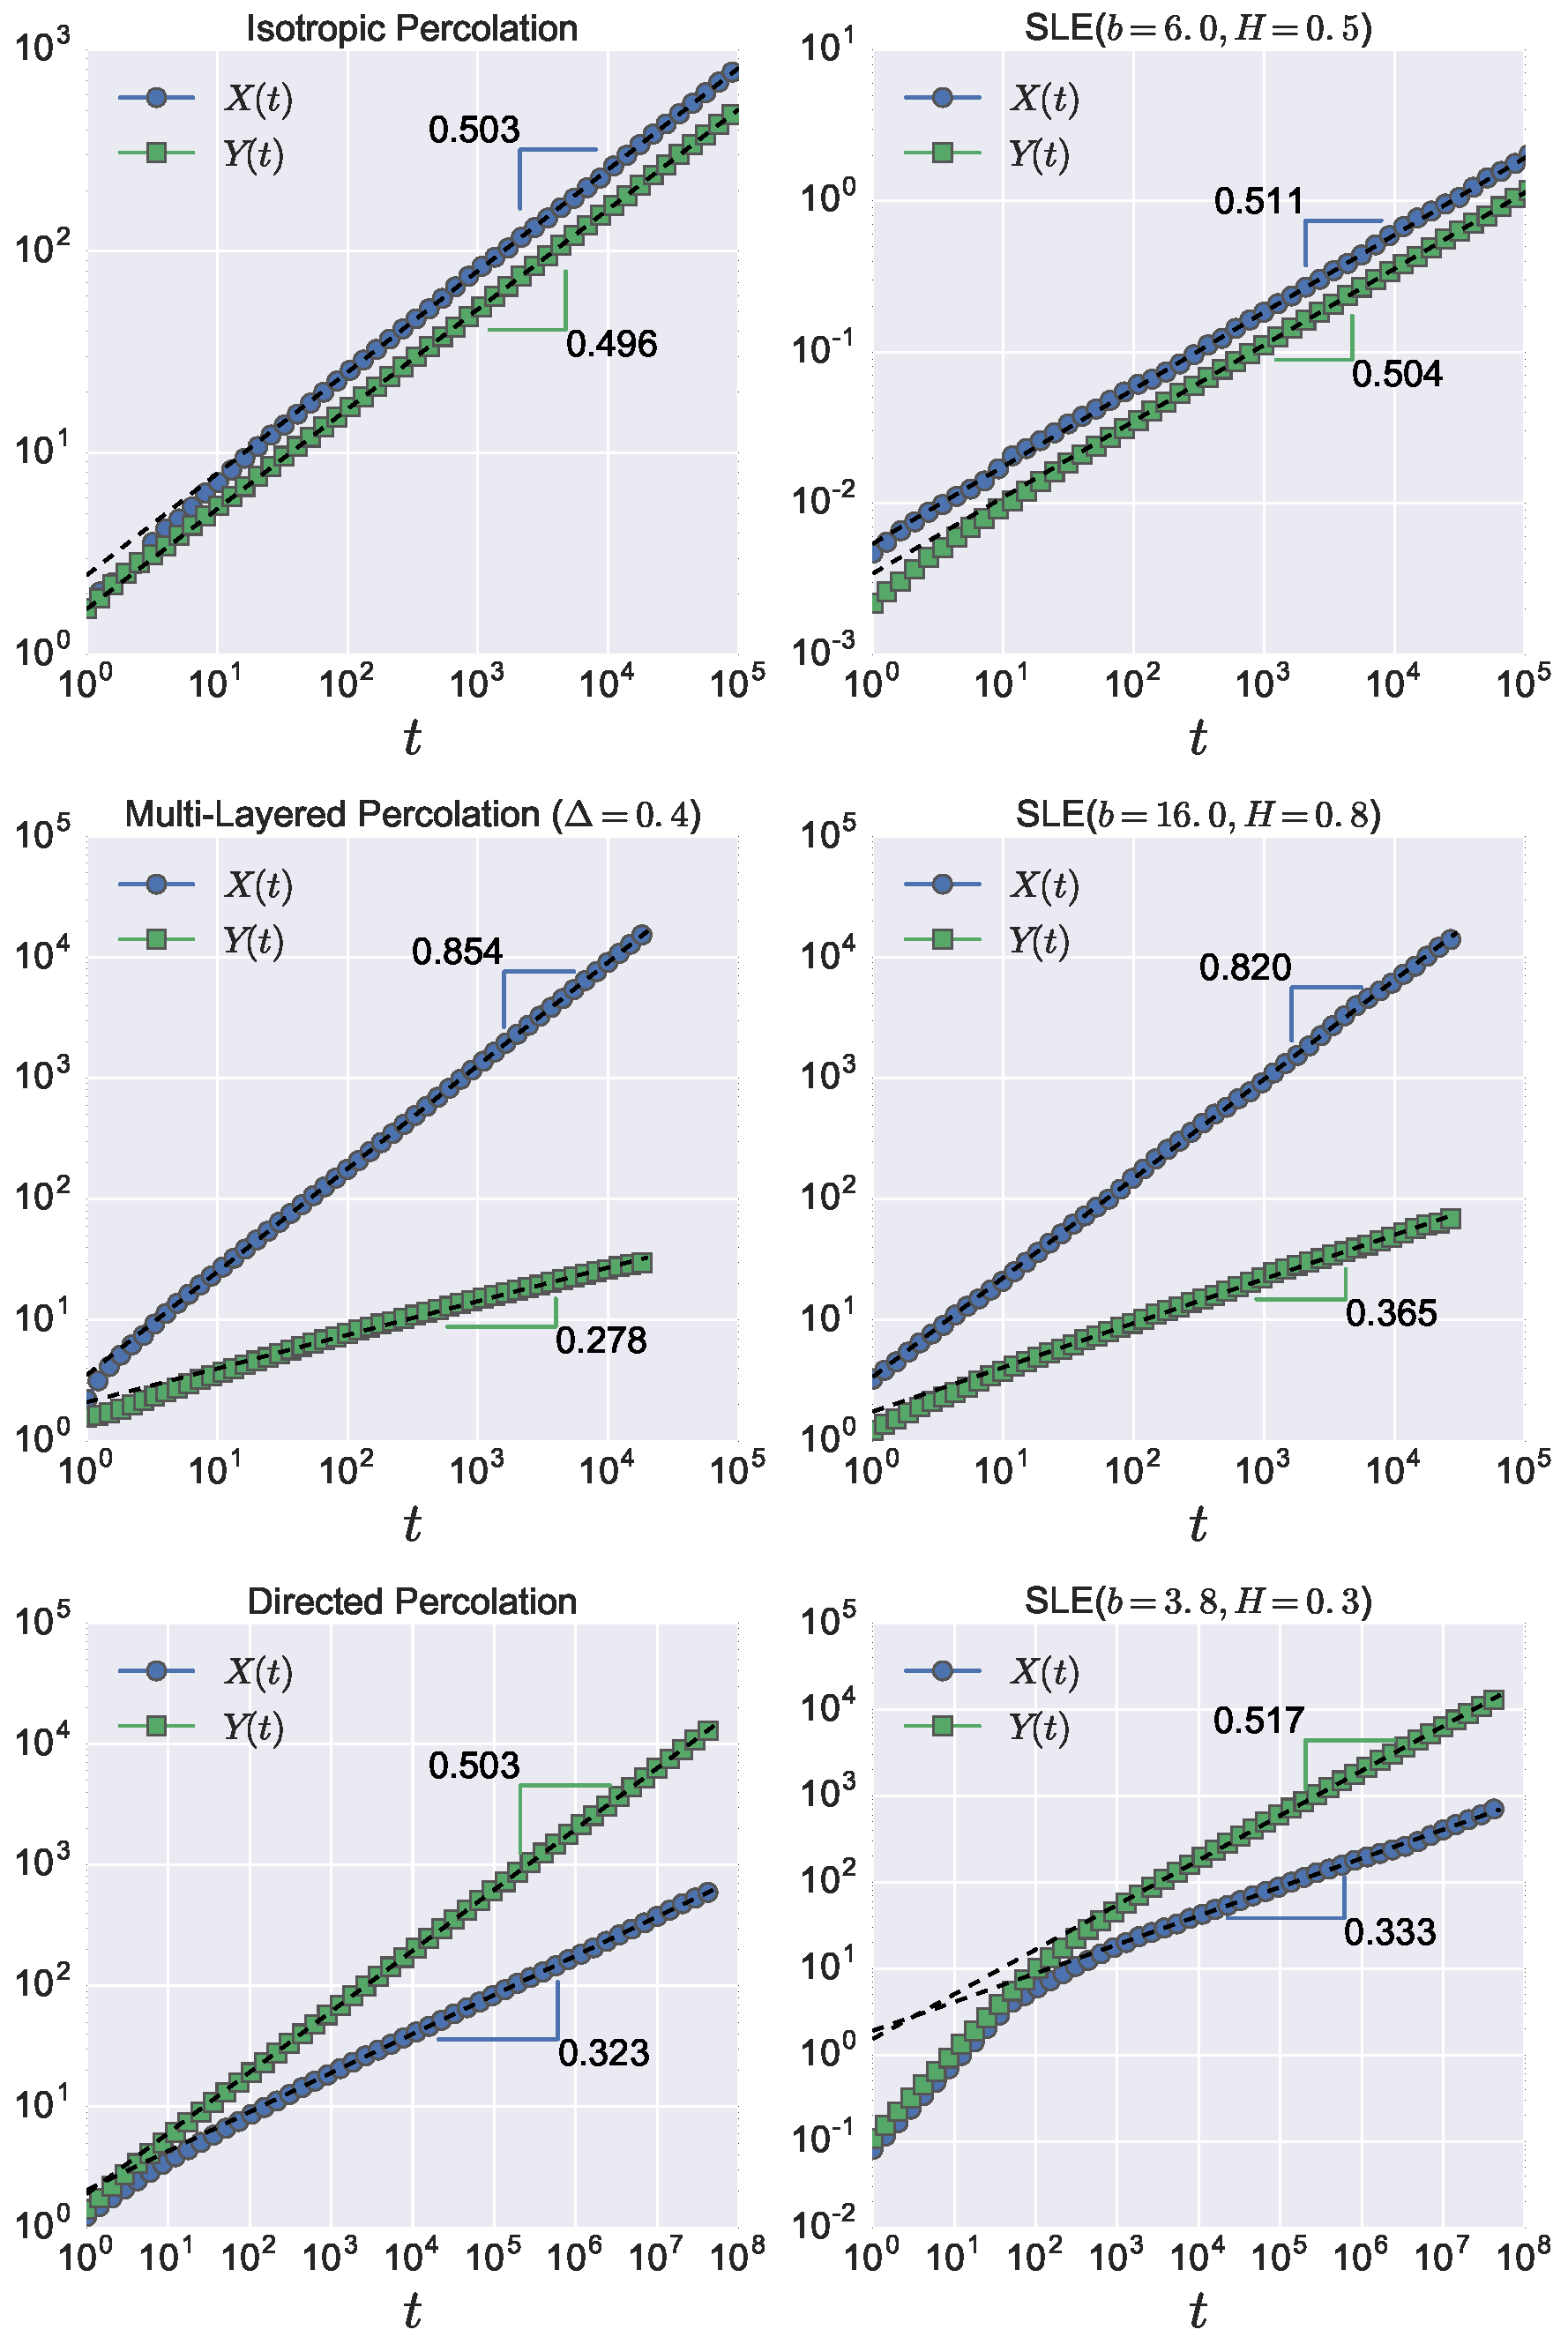
\includegraphics[scale=0.45]{chapters/ch6-asle/figs/timescaling}
\end{center}
\caption{Scaling analysis of the percolation models and their SLE equivalents.
    Here we observe how the total width, $X(t)$, and and height, $Y(t)$, of the
    traces evolve in time. According to the SLE time.}
\label{fig:timescaling}
\end{figure}



\begin{figure}
\begin{center}
    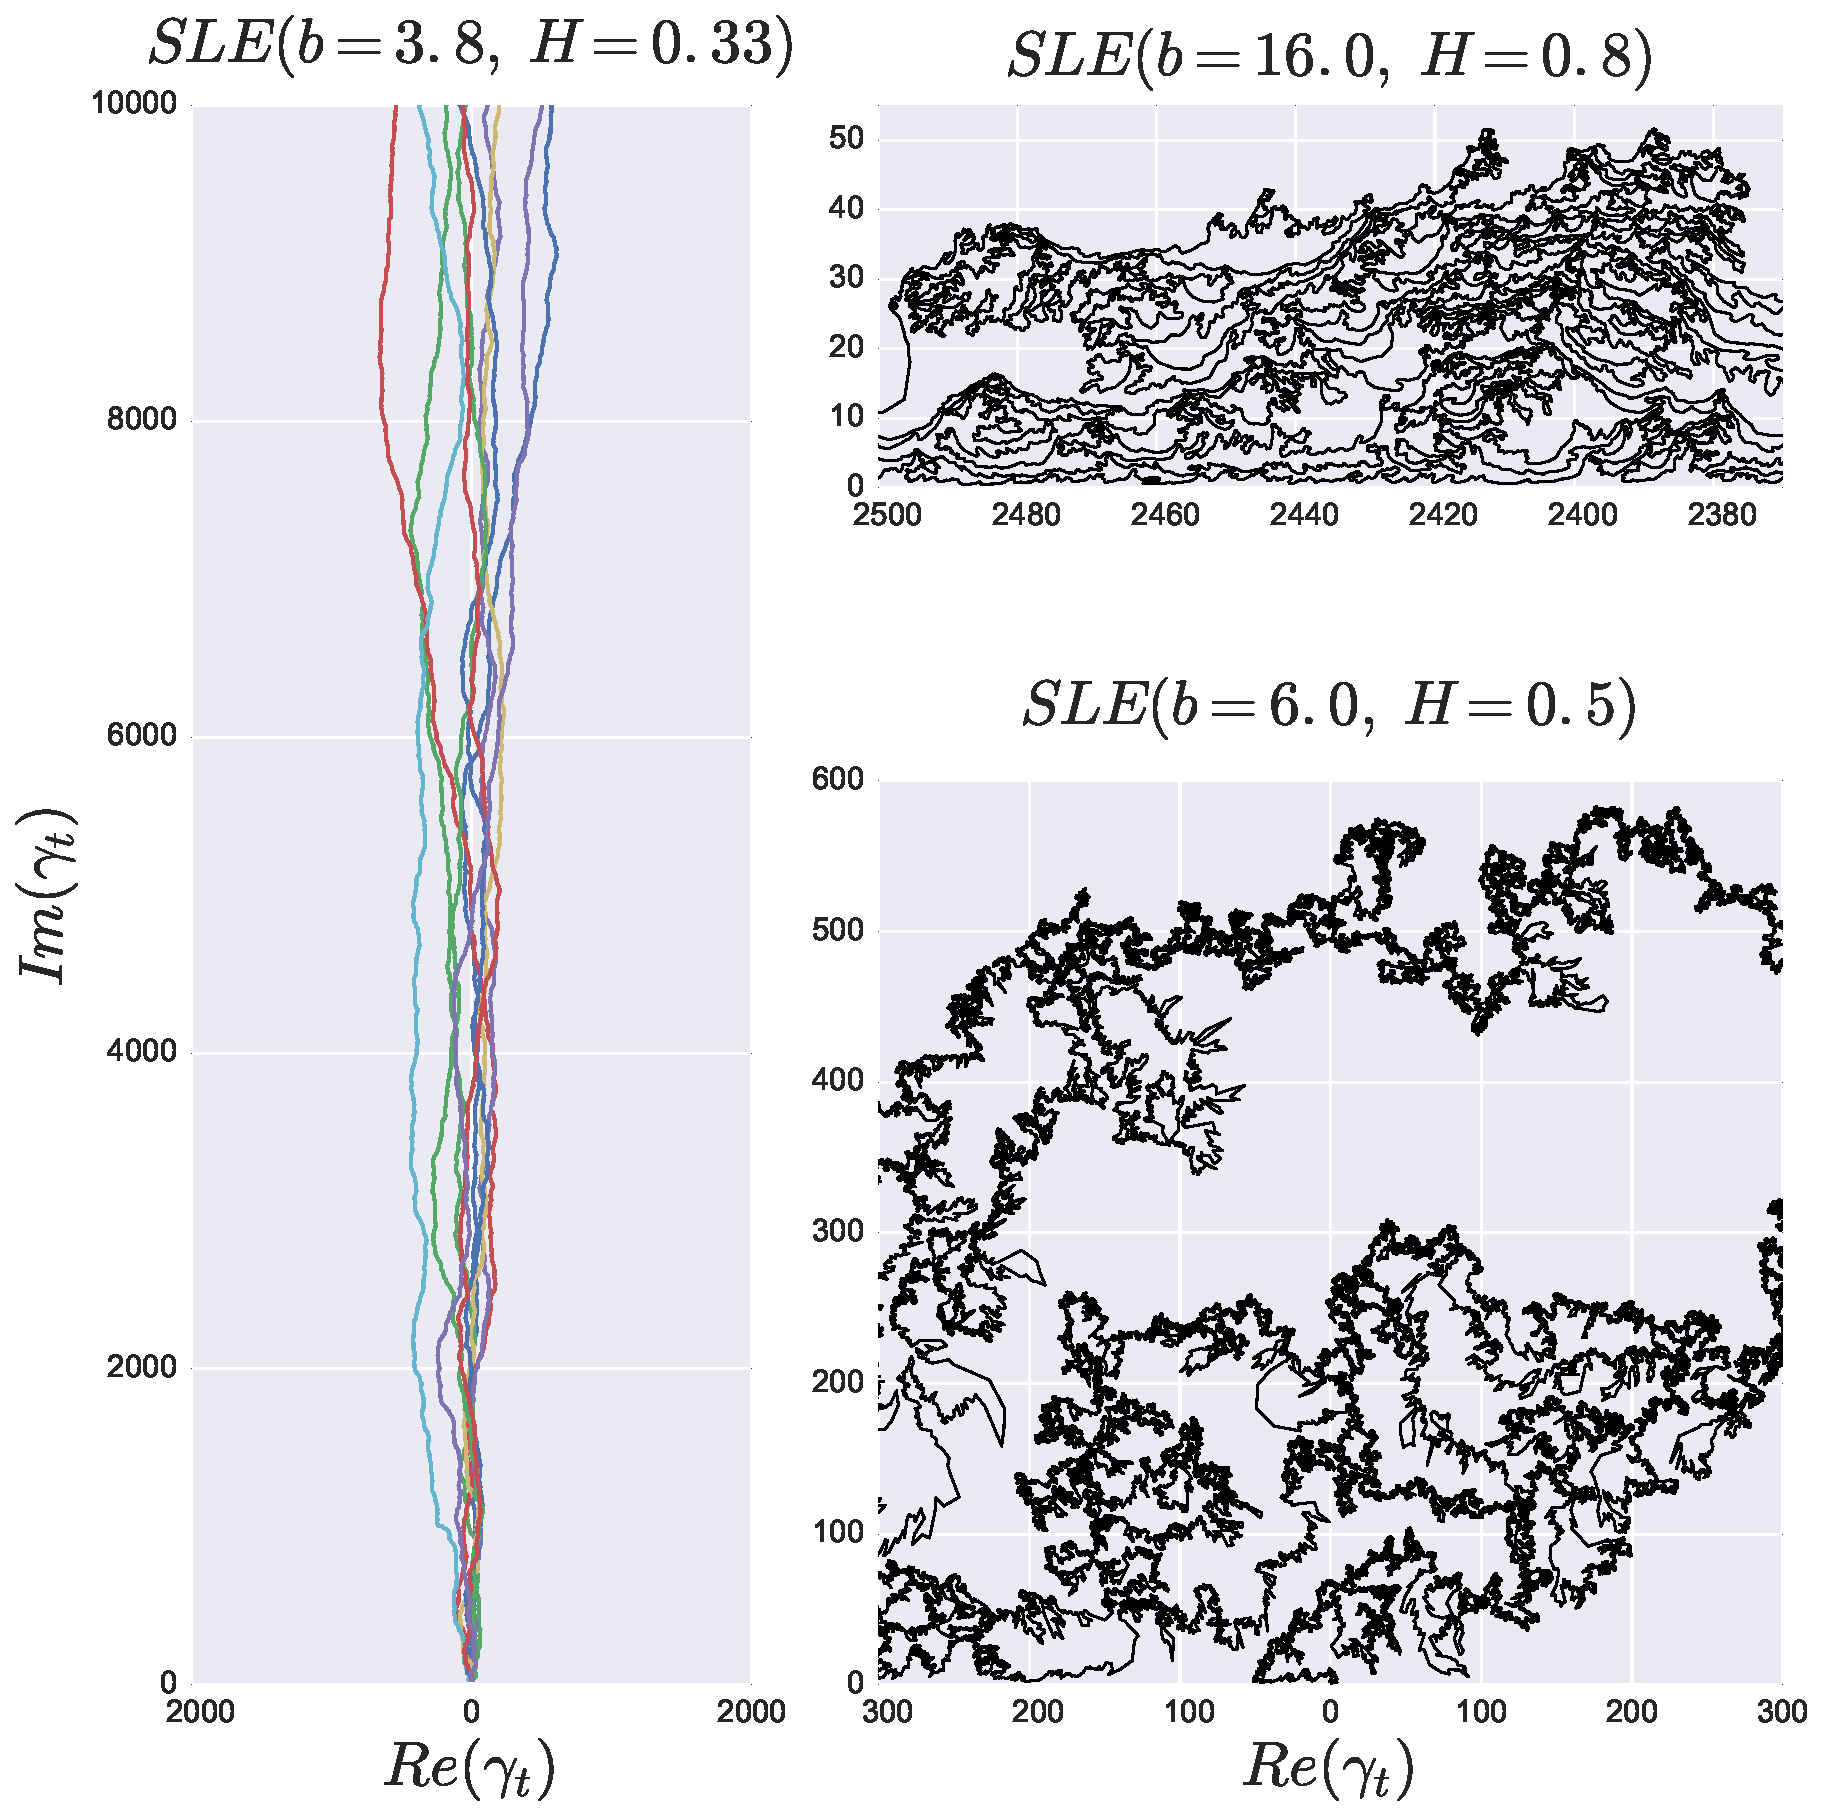
\includegraphics[scale=0.5]{chapters/ch6-asle/figs/asle_traces}
\end{center}
\caption{Examples of $SLE(b,H)$ generate using the three sets of parameters
    that we drew from the diffusion analysis (Figure~[???]). For the correlated
    ($H>0.5$) and uncorrelated ($H=0.5$) we show one example of each. In the
    anticorrelated we show several instances. We used the zipper algorithm with
    $10^6$ points equally spaced in the interval $t\in[0, t_f]$, where the
    values of $t_f$ used can be found in Table~[???].}
\label{fig:asle_traces}
\end{figure}

\begin{figure}
\begin{center}
    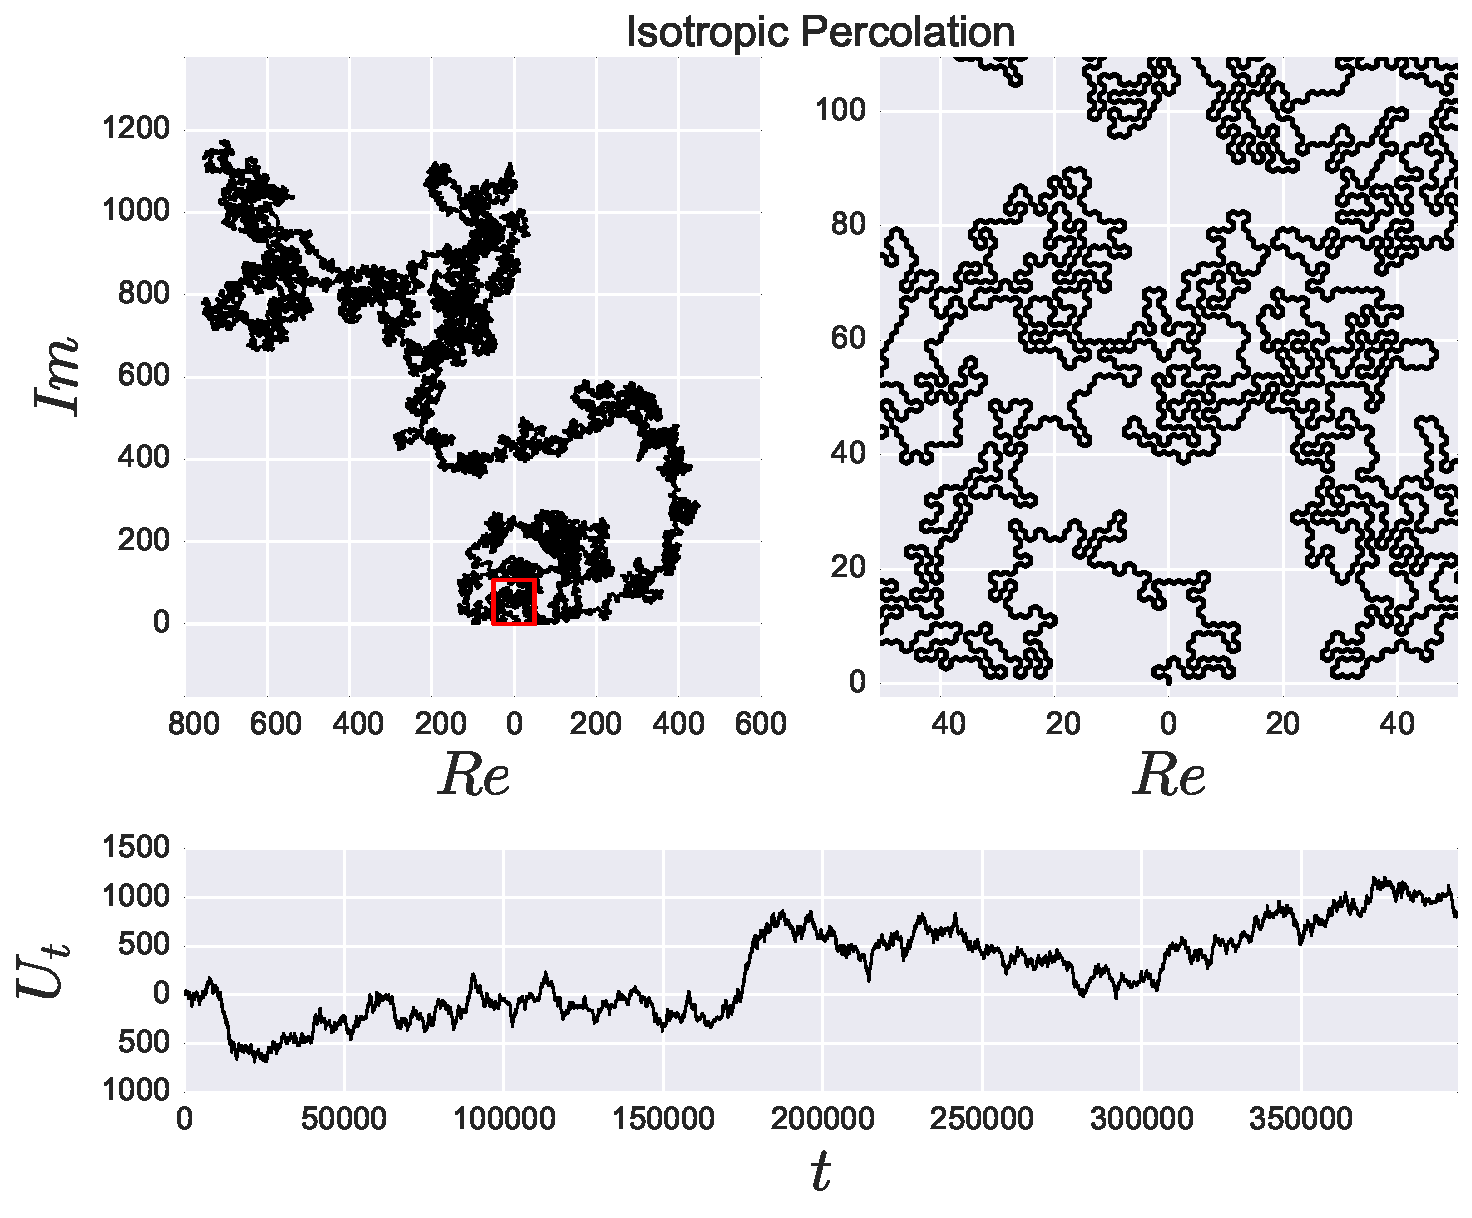
\includegraphics[scale=0.5]{chapters/ch6-asle/figs/ip_trdr}
\end{center}
\caption{Example of a cluster perimeter of the isotropic percolation model in
    the triangular lattice with a detail shown. The bottom graph is the driving
    function obtained by applying the zipper algorithm to this trace.}
\label{fig:ip_trdr}
\end{figure}

\begin{figure}
\begin{center}
    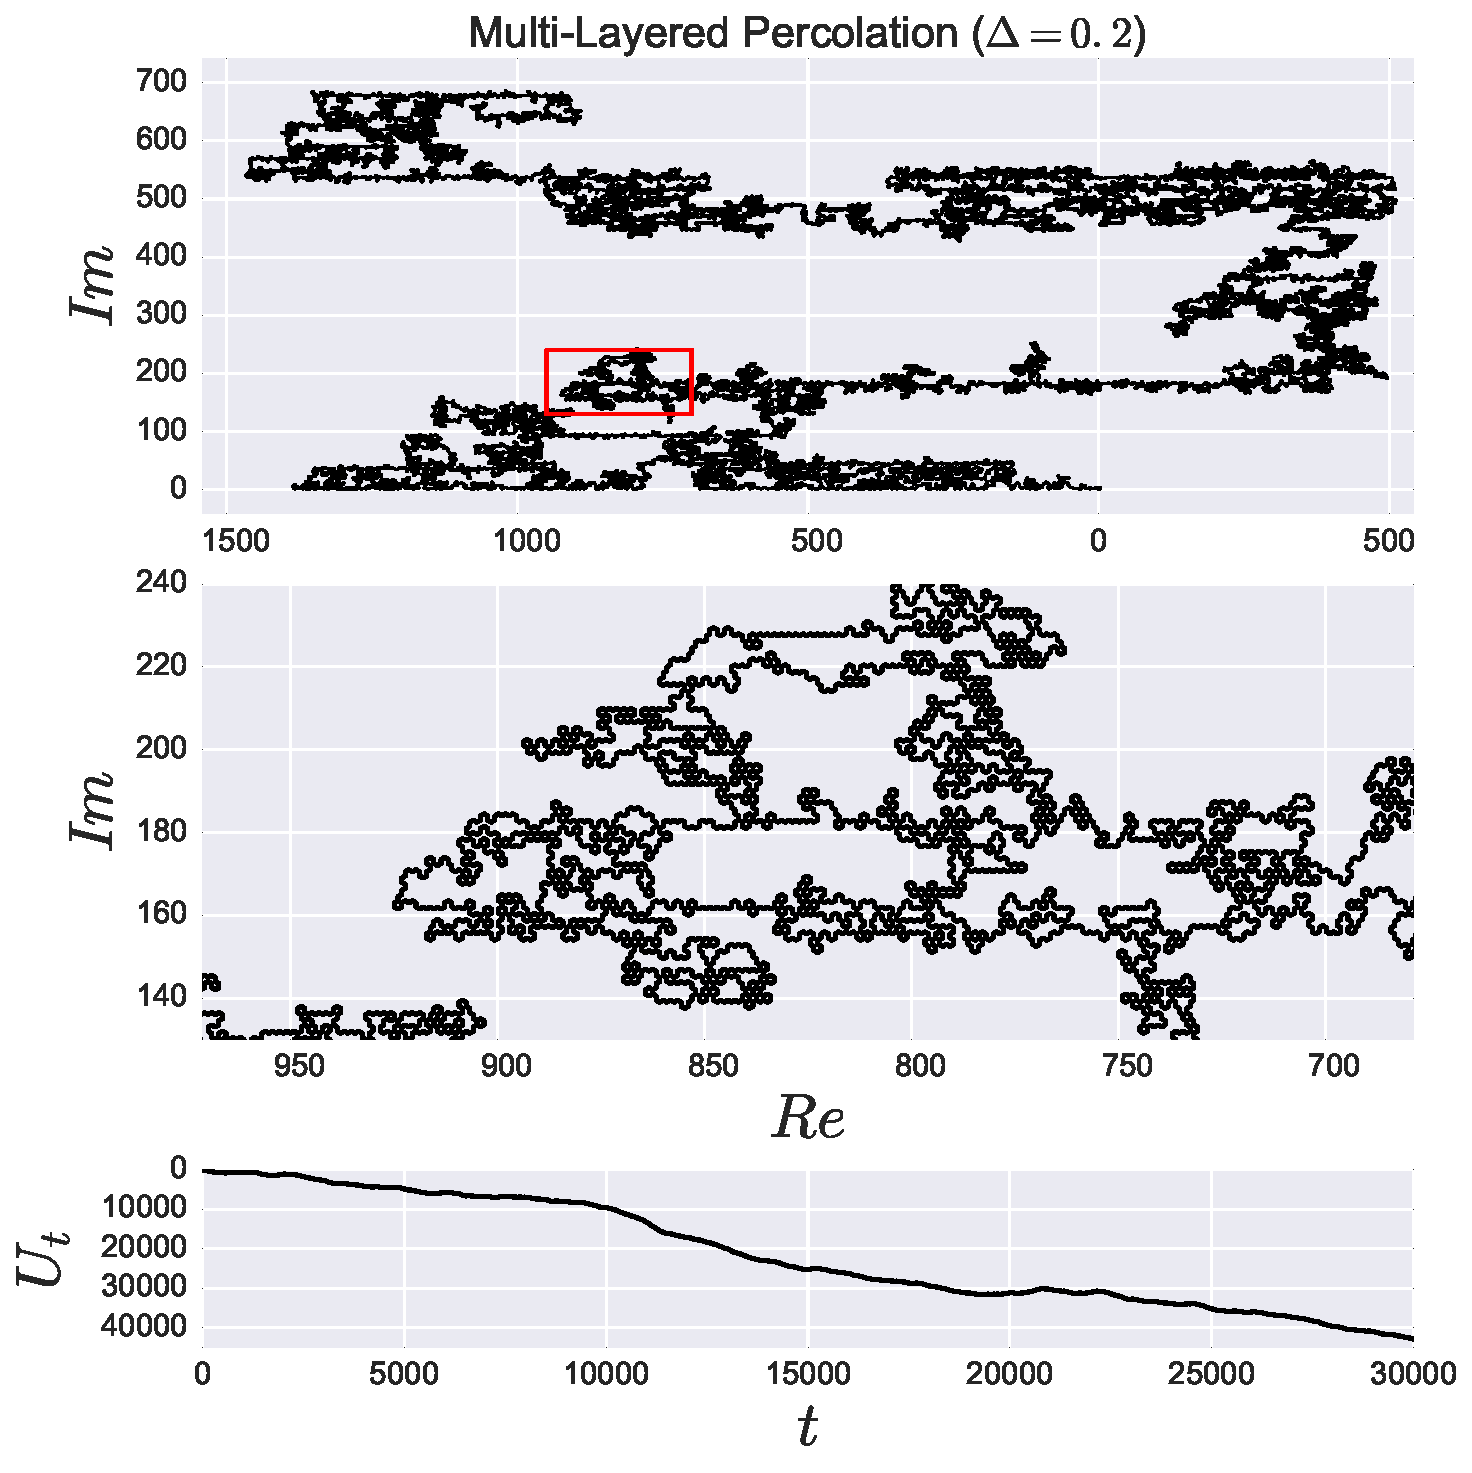
\includegraphics[scale=0.5]{chapters/ch6-asle/figs/ml_trdr}
\end{center}
\caption{Example of a cluster perimeter of the multi-layered percolation model
    in the triangular lattice ($\Delta=0.2$) with a detail shown. The bottom
    graph is the driving function obtained by applying the zipper algorithm to
    this trace.}
\label{fig:ml_trdr}
\end{figure}

\begin{figure}
\begin{center}
    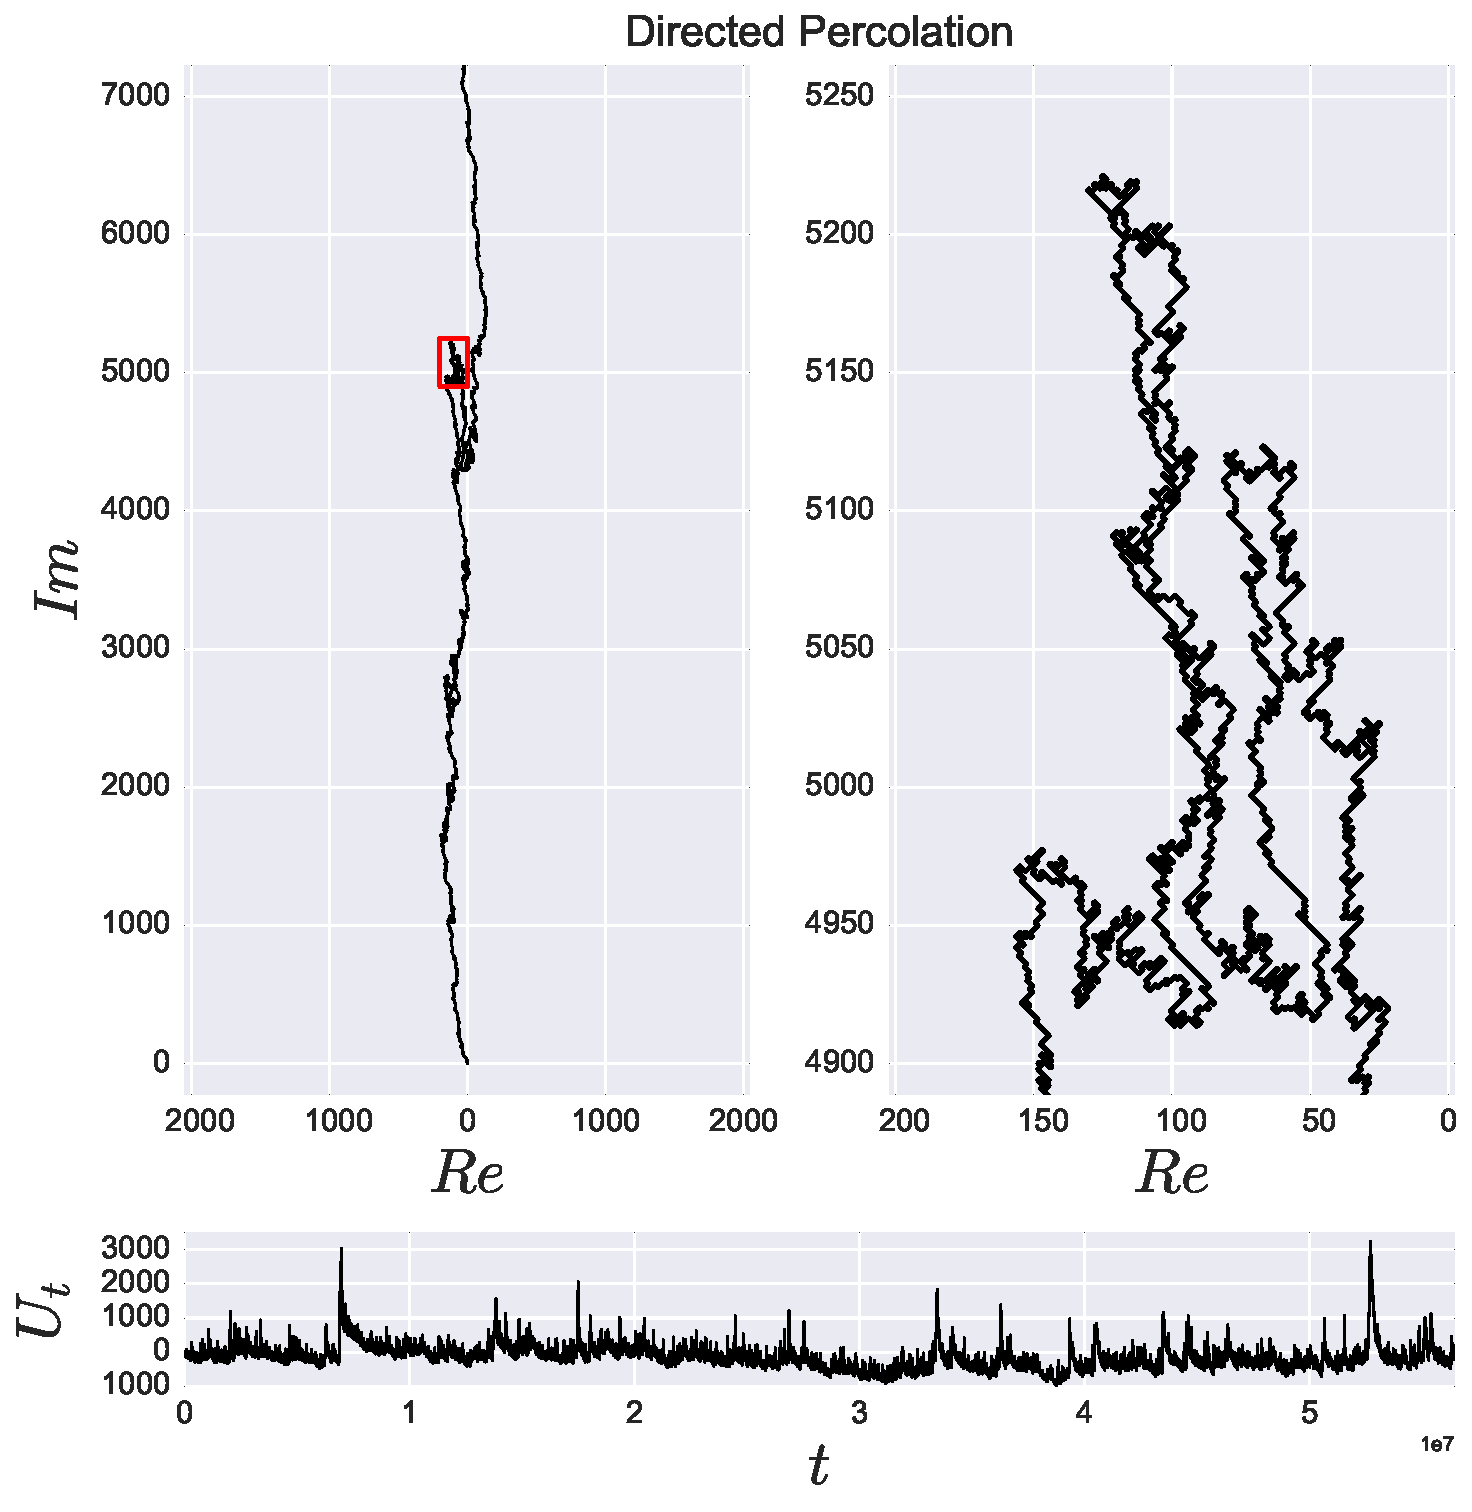
\includegraphics[scale=0.5]{chapters/ch6-asle/figs/dp_trdr}
\end{center}
\caption{Example of a cluster perimeter of the bond directed percolation model
    in the square lattice with a detail shown. The bottom graph is the driving
    function obtained by applying the zipper algorithm to this trace.}
\label{fig:dp_trdr}
\end{figure}

\begin{table}[t]
\newcolumntype{L}[1]{>{\raggedright\let\newline\\\arraybackslash\hspace{0pt}}m{#1}}
\begin{centering}
\begin{tabular}{L{3cm}L{1.5cm}L{1.5cm}L{1.5cm}L{1.5cm}L{1.5cm}L{1.5cm}}
\bottomrule[0.1mm]
\toprule[0.1mm]
                   & $H$    & $b$    & $t_{f}$         & $N$      & $M$      & $\ell_{max}$    \\
\bottomrule[0.1mm]
Ensemble 1         & $0.5$  & $6.0$  & $2\times10^{5}$ & $10^{6}$ & $10^{5}$ & $2\times10^{4}$ \\
Ensemble 2         & $0.8$  & $16.0$ & $3\times10^{4}$ & $10^{6}$ & $10^{5}$ & $8\times10^{4}$ \\
Ensemble 3         & $0.33$ & $3.8$  & $5\times10^{7}$ & $10^{6}$ & $10^{5}$ & $2\times10^{4}$ \\
\bottomrule[0.1mm]
\toprule[0.1mm]
\end{tabular}
\end{centering}
\caption{Simulation parameters used to generate the SLE traces. $H$ is the
    Hurst exponent and $b$ is the diffusion coefficient of the fractional Brownian
    motion used as driving function. The curves were computed for $N$ times $t_i$
    equally spaced in the interval $[0, t_f]$. The resulting trace is
    reparametrized as a function of its length and interpolated in $M$ points
    equally spaced in the interval $[0,\ell_{max}]$.}
\label{tab:param}
\end{table}


